  \documentclass{beamer}
  \usepackage[utf8]{inputenc}
  \usepackage{eurosym}
  \usetheme{marburg}
  \usefonttheme{serif}

\subtitle{Impact de l'activité professionnelle sur le santé perçue des sujets de EPP3}
  \title{Soutenance de stage \\ M1 Mathématiques en interaction}
  \author{Odélia Guedj\\ Encadrant: J.P. Empana (MD,PhD)}
  \institute{Université Paris Saclay (UEVE) / INSERM U970 E04 }
  
  \titlegraphic{
\includegraphics[width=3cm]{logo_inserm.jpg}\hspace*{1cm}~%
   
\includegraphics[width=1cm]{logo_parcc.jpg}\hspace*{1cm}~%
   
\includegraphics[width = 3cm]{logo_ueve_saclay.png}
}

\setbeamercolor{titre}{bg=blue,fg=white}
\setbeamercolor{texte}{bg=blue!10,fg=black}

\begin{document}

\frame{\titlepage}

\section*{Sommaire}
\begin{frame}
\frametitle{Table des matières}
  \tableofcontents
\end{frame} 

\section{Contexte}
\subsection{Inserm U970 E04}

\begin{frame}
\frametitle{Inserm U970}


\pause
\begin{beamerboxesrounded}[upper = titre, lower = texte, shadow = true]{INSERM U970 E04}
\pause
Integrative Epidemiology of Cardiovascular Desease
\end{beamerboxesrounded}

\pause
\begin{beamerboxesrounded}[upper = titre, lower = texte, shadow = true]{Où ?}
\pause
Bâtiment recherche de l'HEGP\\
56 rue Leblanc 75015
\end{beamerboxesrounded}

\pause
\begin{beamerboxesrounded}[upper = titre, lower = texte, shadow = true]{Qui ?}
\pause
\begin{itemize}
\item Dr J.P. Empana (MD,PhD) (Santé Publique)
\pause
\item Dr X. Jouven (MD,PhD) (Cardiologie)
\end{itemize}
\end{beamerboxesrounded}

\pause
\begin{beamerboxesrounded}[upper = titre, lower = texte, shadow = true]{Quoi ?}
\pause
\begin{itemize}
\item CEMS : Centre d'Expertise de Mort Subite
\pause
\item Étude des maladies cardiovasculaires en Afrique
\pause
\item EPP3 : Étude Parisienne Prospective 3 
\end{itemize}
\end{beamerboxesrounded}
\end{frame}

\begin{frame}
\frametitle{Fonctionnement interne}

\begin{itemize}
\pause
\item Équipe d'une quarantaine de personnes: Médecins, ARC, Statisticiens, thésards...
\pause
\item Chaque semaine : séminaire organisé par l'une des équipes de l'U970 (biologie expérimentale, épidémiologie, médecine).
\pause
\item Réunions régulières: 
\begin{itemize}
\pause
\item Méthodologie
\pause
\item Lecture critique d'articles
\pause
\item Avancée des études: récupération des données, problèmes à la saisie, suivi des sujets...
\end{itemize}
\end{itemize}
\end{frame}


\subsection{EPP3}
\begin{frame}
\frametitle{Étude Parisienne Prospective 3}

\pause
\begin{beamerboxesrounded}[upper = titre, lower = texte, shadow = true]{But}
\pause
Étude de nouveaux paramètres de fréquence cardiaque, sensibilité du baroréflexe et risque de mort subite.
\end{beamerboxesrounded}

\pause
\begin{beamerboxesrounded}[upper = titre, lower = texte, shadow = true]{Inclusion des sujets}
\pause
Patients IPC entre 50 et 75 ans recrutés entre 2008 et 2011.
\end{beamerboxesrounded}

\pause
Constitution de la base de données:\\
\begin{itemize}
\pause
\item Suivi sur 20 ans: 1 questionnaire tous les deux ans.
\pause
\item Système de validation d'événements cardiovasculaires déclarés par les patients: récupération de comptes rendus hospitaliers dans les hôpitaux.
\pause
\item n = 10 157 (Hommes = 60 $\%$)
\end{itemize}
\end{frame}




\subsection{Sujet de stage}

\begin{frame}
\frametitle{Sujet de stage}

\pause
\begin{beamerboxesrounded}[upper = titre, lower = texte, shadow = true]{Sujet}
\pause
Étude de l'impact de l'activité professionnelle sur les individus de l'étude EPP3.\end{beamerboxesrounded}

\pause
\begin{beamerboxesrounded}[upper = titre, lower = texte, shadow = true]{La santé perçue}
\pause
\begin{itemize}
\item Le sujet auto-évalue sa santé sur une échelle de 0 à 11.
\pause
\item Très bon indicateur de mortalité: permet de rendre compte de la santé \textit{globale} des individus en incluant une part subjective non mesurable par les examens médicaux usuels.
\pause
\item \textit{Self-rated health before and after retirement in France (GAZEL) : a cohort study.
\tiny{Hugo Westerlund, Mika Kivimäki, Archana Singh-Manoux, Maria Melchior, Jane E. Ferrie,
Jaana Pentti, Markus Jokela, Constanze Leineweber, Marcel Goldberg, Marie Zins, and Jussi
Vahtera.} 
Lancet (London, England)}
\end{itemize}
\end{beamerboxesrounded}

\end{frame}

\section{Méthodes}
\subsection{Variables}

\begin{frame}
\frametitle{Variables}

\pause
\begin{beamerboxesrounded}[upper = titre, lower = texte, shadow = true]{Variable d'intérêt}
\pause
Santé perçue binarisée (0-7: bon, 8-10: mauvais)
\end{beamerboxesrounded}

\pause
\begin{beamerboxesrounded}[upper = titre, lower = texte, shadow = true]{Variable d'exposition}
\pause
Activité professionnelle
\end{beamerboxesrounded}

\pause
\begin{beamerboxesrounded}[upper = titre, lower = texte, shadow = true]{Autres variables}
\pause
Sexe, situation familiale, âge, éducation, catégorie socio-professionnelle, indice de masse corporelle, tabac, diabète, activité sportive, hypertension artérielle, consommation d'alcool, score de précarité, score de stress perçu, dépression.
\end{beamerboxesrounded}

\end{frame}

\begin{frame}
\frametitle{Description de la population d'étude}

\pause
Variables de style de vie:\\
\pause
\begin{center}
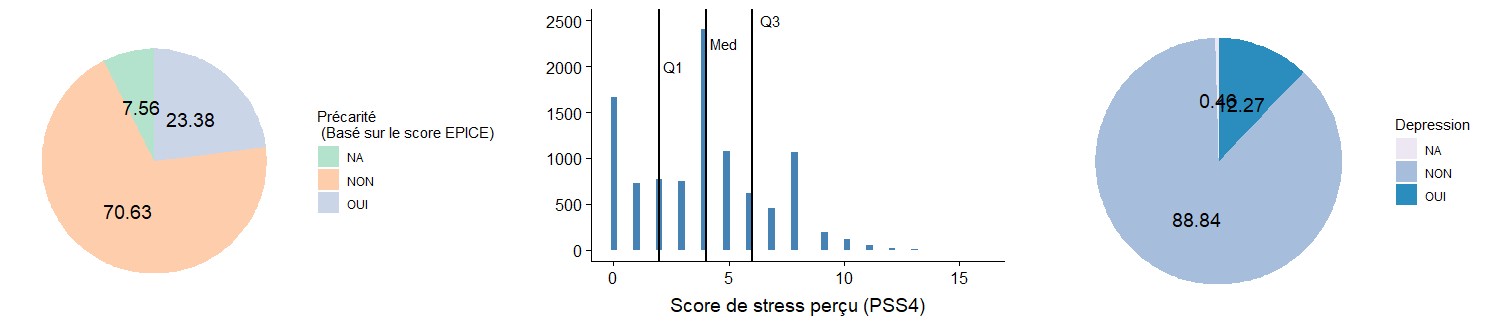
\includegraphics[width = 5.5cm]{tab_var_sante_psy.png}\\
\end{center}

\pause
Variables socio-administratives:\\
\pause
\begin{center}
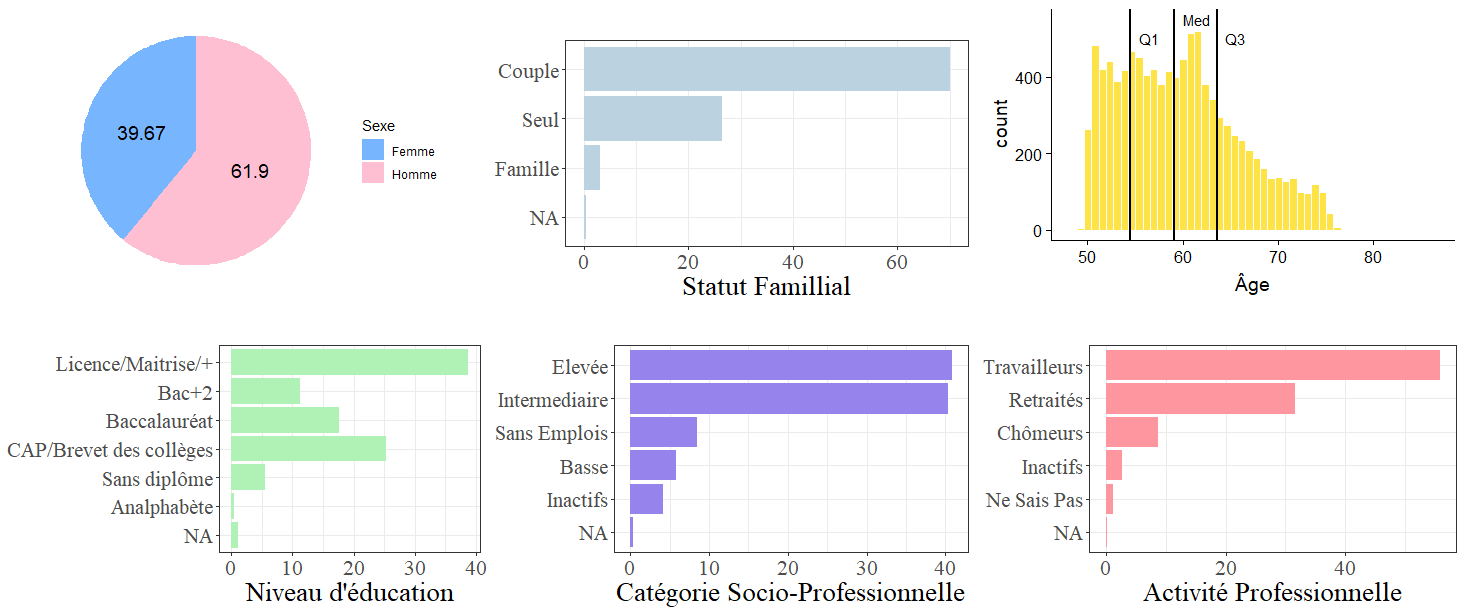
\includegraphics[width = 5.5cm]{tab_var_socio_ad.png}\\
\end{center}

\pause
Variables de santé psychologique:\\
\pause
\begin{center}
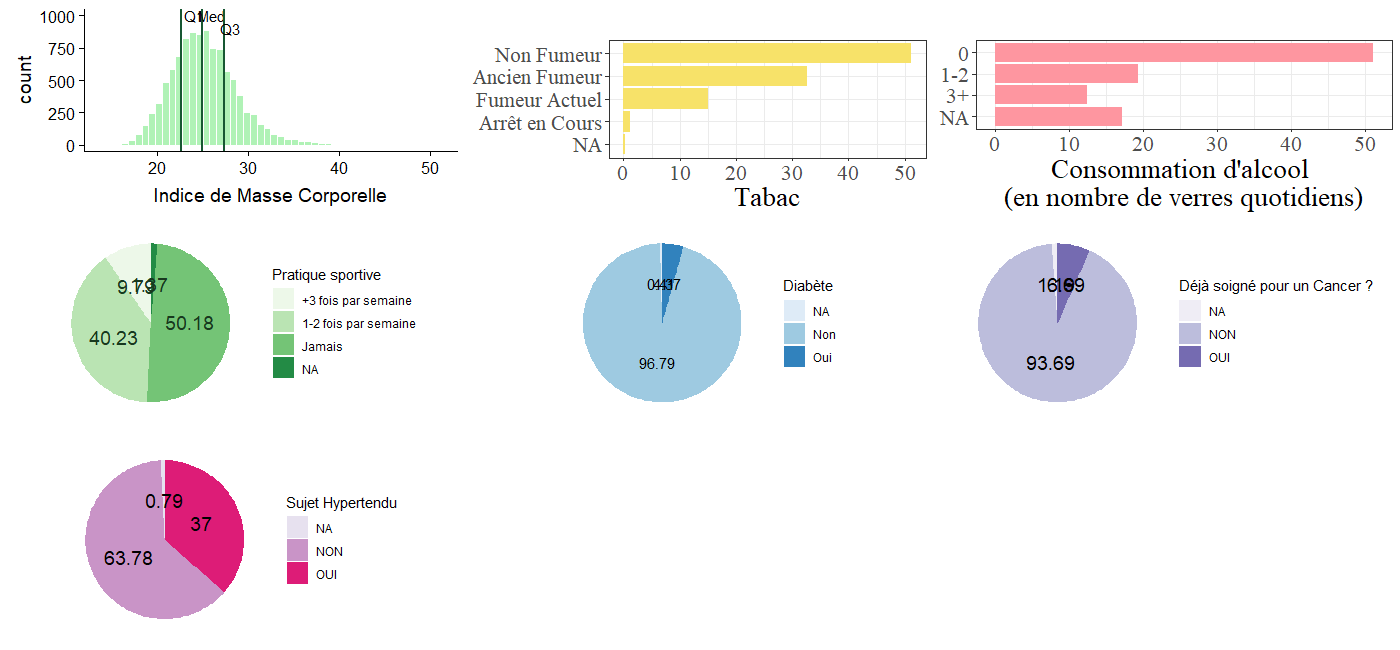
\includegraphics[width = 5.5cm ]{tab_var_sante_phys.png}\\
\end{center}

\end{frame}
\subsection{Construction de la variable d'exposition}
\begin{frame}
\frametitle{Variable d'exposition: activité professionnelle}
\begin{itemize}
\pause
\item Regroupement de l'information de quatre variables différentes en une seule en effectuant une classification manuelle et algorithmique.
\pause
\item Classification algorithmique avec une ACM et une CAH qui identifie 4 groupes:
\end{itemize}
\pause
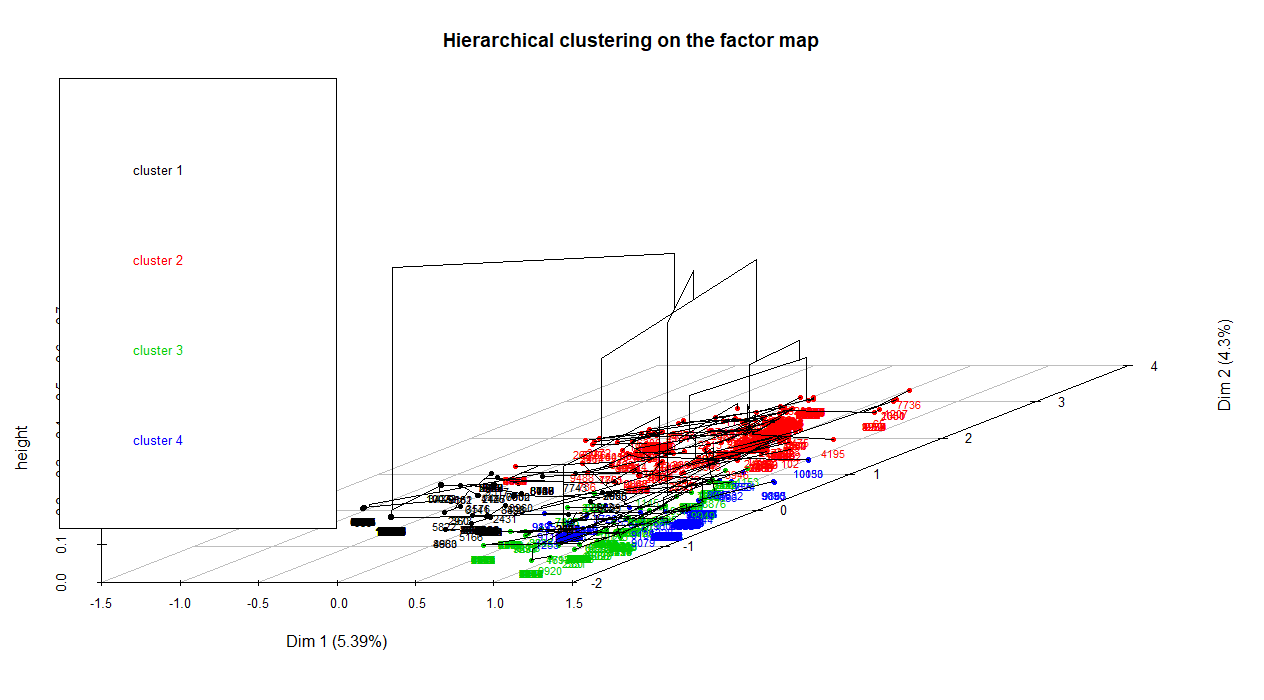
\includegraphics[width = 10cm]{map_cah.png}
\end{frame}
\begin{frame}
\frametitle{Analyse de la Classification Ascendante Hiérarchique}
\begin{itemize}
\pause
\item
Seuls 5 $\%$ des individus sont classés différemment dans les deux classifications.
\pause
\item
Cependant , un test du $\chi^2$ nous indique que les deux classifications ne sont pas significativement similaires, on retient la variable classée manuellement comme variable d'exposition.
\end{itemize}
\begin{center}
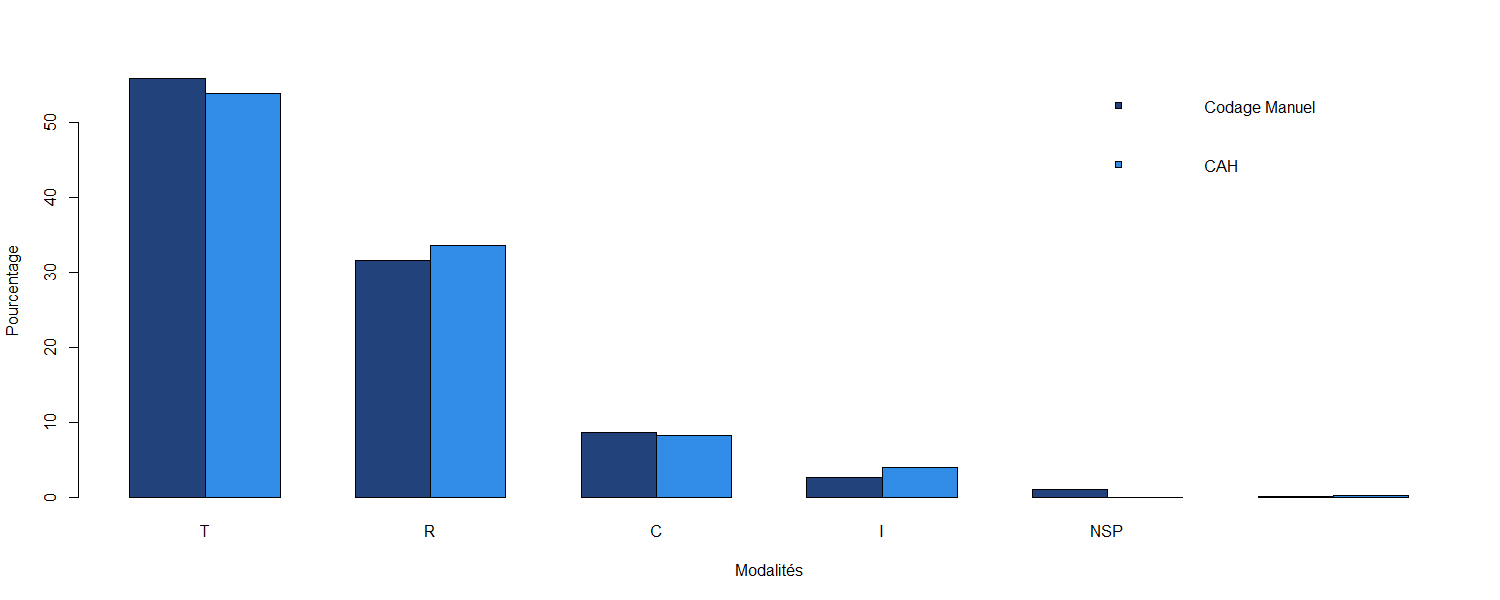
\includegraphics[width = 8cm]{comp_codages_activpro_pourcentage.png}
\end{center}
\end{frame}

\section{Résultats}
\subsection{Flowchart}

\begin{frame}
\frametitle{Flowchart}
\pause
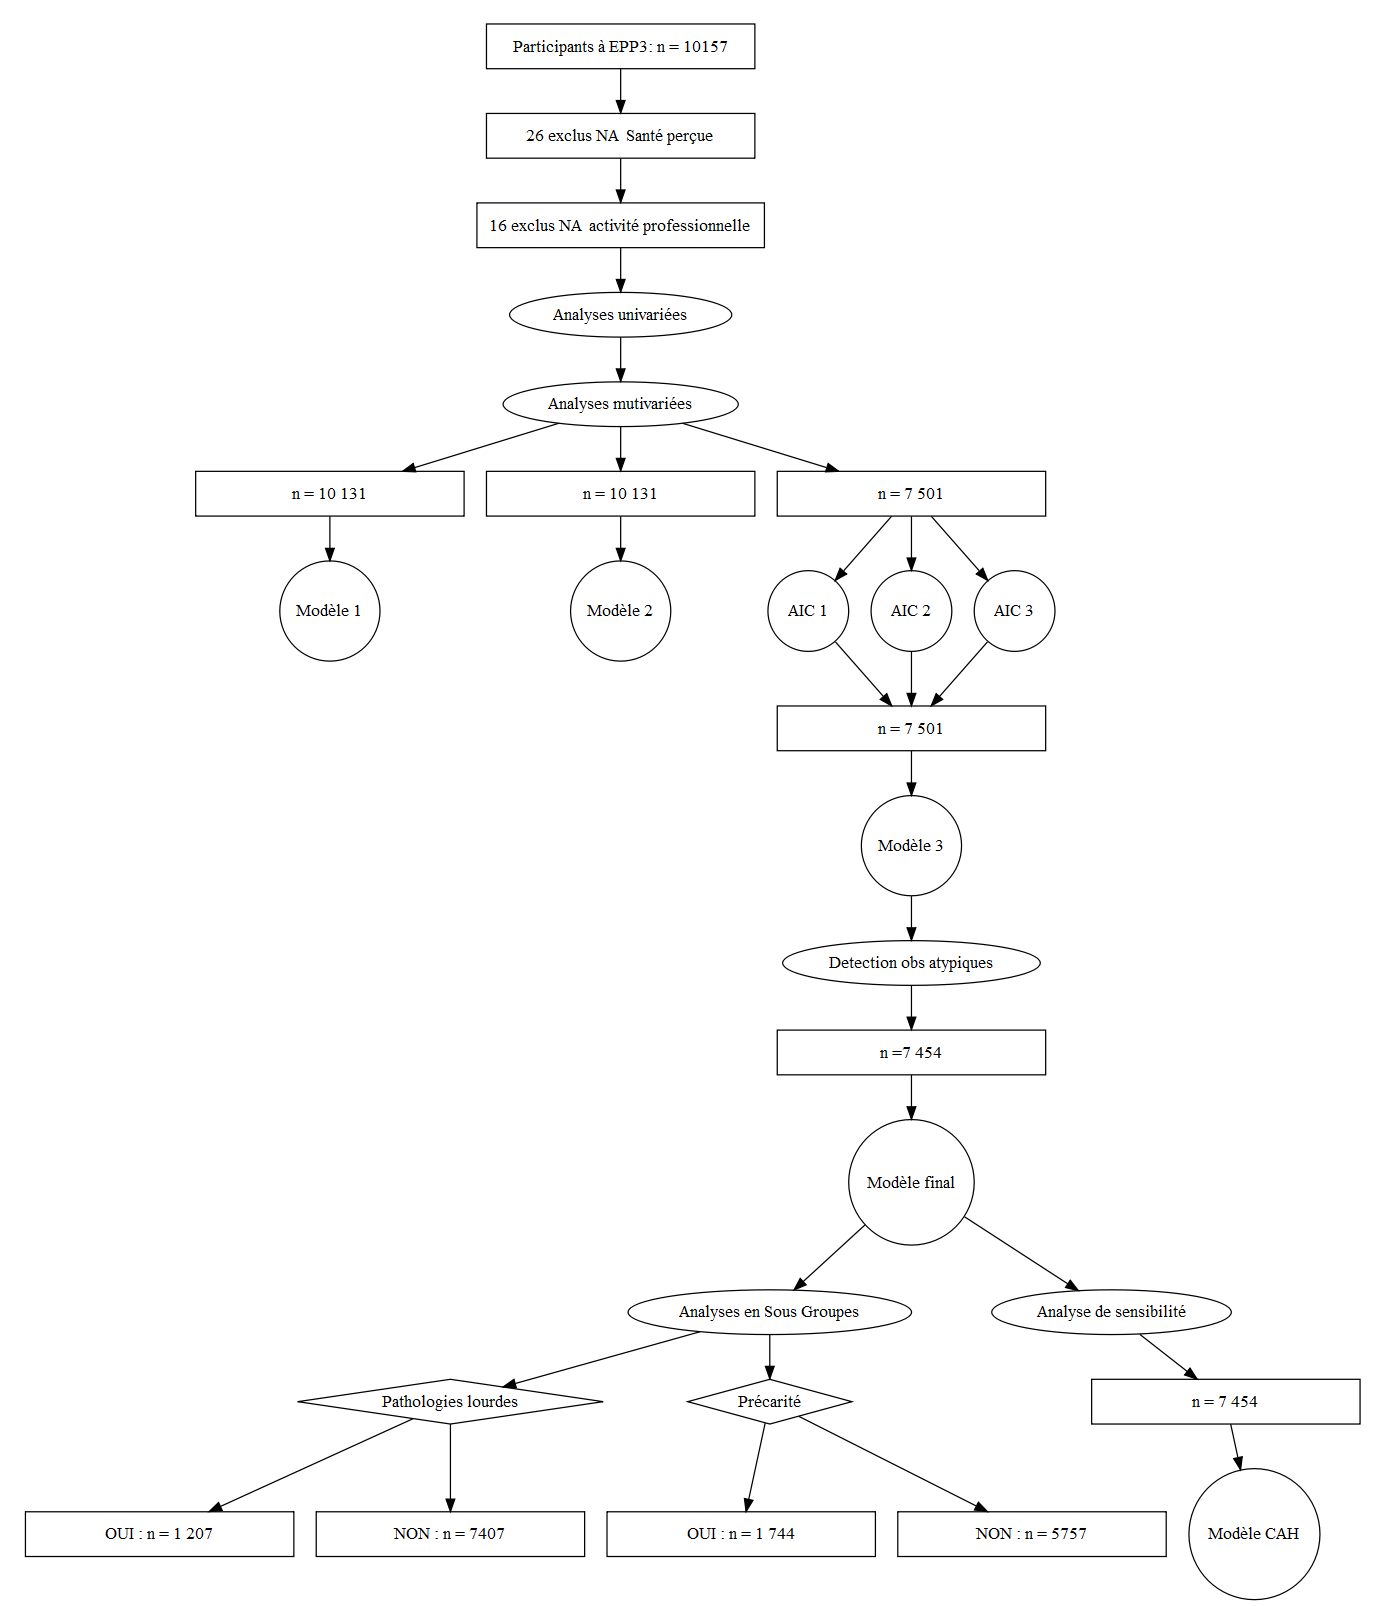
\includegraphics[width = 7.5cm]{flowchart.png}
\end{frame}


\subsection{Modèle final}
\begin{frame}
\frametitle{Résultats}
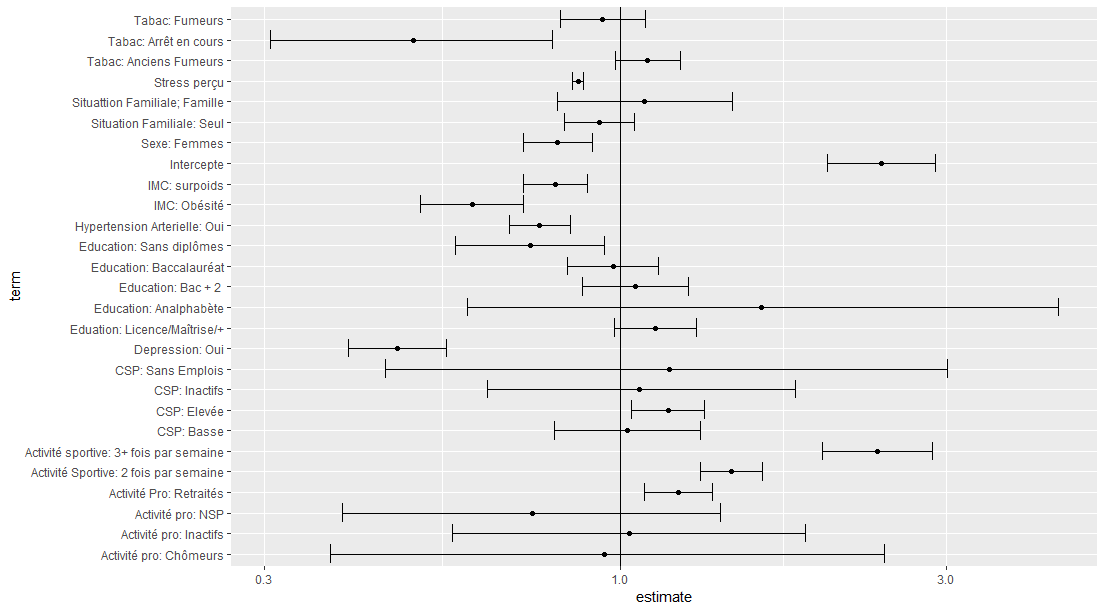
\includegraphics [width = 10cm, height = 8.8cm]{plot_model_final.png}
\end{frame}

\section{Retour d'expérience}
\subsection{L'épidémiologie}
\begin{frame}
\frametitle{Découverte de l'épidémiologie}
\begin{enumerate}
\pause
\item Discipline passionnante entre la médecine et les statistiques.
\pause
\item Perspectives différentes des Statistiques théoriques: 
\begin{itemize}
\pause
\item Pertinence clinique
\pause
\item Hypothèses (normalité, linéarité, résidus) pas toujours respectées
\pause
\item Méfiance vis à vis de nouveaux outils (Conférence de la SFT: utilisation de l'IA en santé)
\end{itemize} 
\end{enumerate}
\end{frame}

\subsection{Le monde de la recherche}
\begin{frame}
\frametitle{Découverte du monde de la Recherche}
\begin{itemize}
\pause
\item Travail d'équipe: brassage d'idées et de points de vues
\pause
\item Travail de bibliographie: Non libre accès aux articles scientifiques !!
\pause
\item Importance de la bonne communication: collaborations, partage des données...
\pause
\item PubMed/Zotero/BibTex/GitHub
\end{itemize}
\end{frame}

\section{Remerciements}
\begin{frame}
\frametitle{Remerciements}
\bigskip
\begin{center}
Merci pour votre écoute !
\end{center}
\bigskip
\bigskip
\bigskip
\bigskip
\bigskip
\bigskip
\bigskip
\begin{flushright}
Odélia Guedj\\
M1 MINT\\
\end{flushright}
\end{frame}

\end{document}
